\chapter{Speciální instance}
V této kapitole se podíváme na omezené instance klastrové rovinnosti. Klastrová rovinnost se dá omezit dvěma způsoby. Jednak omezením, jaké grafy budeme uvažovat, a jednak omezením klastrové hierarchie. První omezenou třídou klastrových grafů jsou kružncice s klastry velikosti 2 a druhou třídou budou cesty s klastry velikosti 2. Uvedeme věty o počtu zakázaných minorů.

\section {Kružnice s klastry velikosti 2}
Hlavním výsledkem této části je výsledek ukazující, že jediným zakázaným minimálním minorem pro kružnice s klastry velikosti 2 je šesticyklus se třemi klastry, kde se vrcholy střídají v jakém klastru jsou (viz následující obrázek). Výsledek je jak pro nakreslenou, tak i nenakreslenou verzi.

\begin{figure}[H]
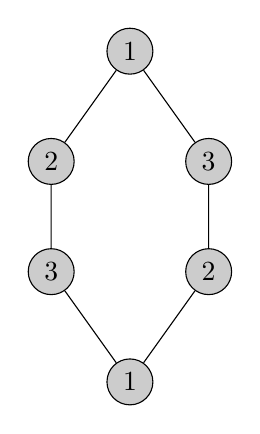
\begin{tikzpicture}[node/.style={circle,fill=black!20,draw,minimum size=1em,inner sep=3pt]}]

    \node[node] (1) at (0,0) {1};
    \node[node] (2) at (-1, -1.4)  {2};
    \node[node] (3) at (-1, -2.8) {3};
    \node[node] (4) at (0,-4.2) {1};
    \node[node] (5) at (1, -2.8)  {2};
    \node[node] (6) at (1, -1.4) {3};

    \draw (1) -- (2) -- (3) -- (4) -- (5) -- (6) -- (1);
\end{tikzpicture}
\caption{Čísla označují, do jakého klastru vrchol patří. Dále v textu bude tento graf označován jako  $C_6^Z$, kde Z značí, že se jedná o zakázaný minor}
\label{fig:zak_minor}
\end{figure}

\begin{theorem}
\label{hlavni_veta}
Instance $(G,\mathcal C)$ je klastrově rovinná $\iff$ $(G,\mathcal C)$ neobsahuje $C_6^Z$ jako minor .
\end{theorem}

Před důkazem věty ukážeme, že $C_6^Z$ není klastrově rovninný.

\begin{lemma} 
$C_6^Z$ není klastrově rovinný.
\end{lemma}
\begin{proof}
Důkaz provedeme pro nenakreslenou verzi. Jelikož klastry jsou velikosti 2, můžeme nahrazovat klastry hranami. Nahrazení všech klastrů hranami však vede přímo na $K_{3,3}$. A protože $K_{3,3}$ není rovinný graf, tak nemůže $C_6^Z$ klastrově rovinný. Poslední nahrazení klastru hranou tedy nelze provést
\end{proof}

U kružnice můžou saturátorové hrany vést pouze vnitřkem nebo vnějškem (myšleno v nakreslení). Pro dvě hrany ze saturátoru má smysl se bavit o tom, zda mohou vést na stejné straně kružnice nebo nikoliv. To nás vede k pojmu grafu konfliktů, který reprezentuje konflikty mezi hranami ze saturátoru. 

\begin{defn}
Graf konfliktů je reprezentací konfliktů saturátorových hran, kde vrcholy jsou klastry a hrany představují konfliktní klastry. Klastry $\{x_1, x_2\}$ a $\{y_1, y_2\}$ mají spolu konflikt, pokud se na kružnici vyskytují v následujícím pořádí $x_1 , ..., y_1, ..., x_2, ..., y_2, ...$ . Grak konfliktů pro klastrový graf $(G,\mathcal C)$ budeme značit $GK_{(G,\mathcal C)}$
\end{defn}

Získáme ihned kritérium, kdy kružnice s klastry velikosti 2 je klastrově rovinný graf. Je to právě tehdy, když graf konfliktů je bipartitní. Dokážeme si to jako lemma.

\begin{lemma}\label{lemma_ekv_graf_konf_kl_rov}Kružnice s klastry velikosti 2 je klastrově rovinná právě tehdy, když graf konfliktů je bipartitní.
\end{lemma}
\begin{proof}
Klastr, jenž je tvořen sousedními vrcholy, zjevně nemůže být podle definice s jiným klastrem v konflkitu. Vrchol příslušného klastru v grafu konfilktů je izolovaný. Stačí tedy uvažovat, že vrcholy v klastru nejsou sousedními.

"$\implies$"
Místo klastrů uvažujme hrany saturátoru, ty mohou vést buď vnitřní stěnou kružnice nebo vnější stěnou kružnice. Hrana v grafu konfliktů vede mezi jeho vrcholy právě tehdy pokud saturované hrany příslušných klastrů vedou různými stěnami. To proto, že podle definice konfliktu, kdyby vedly stejnou stěnou, tak by se musely křížit, což by byl spor s tím, že máme klastrové nakreslení. Pokud jako partity označíme klastry, jež vedou buď vnější stěnou (jedna partita) nebo vnitřní stěnou (druhá partita). Izolované vrcholy dáme libovolně někam.

Opačná implikace je ten samý argument jen obrácené pořadí.
\end{proof}

Uvedeme ještě jedno lemma, ukazující vztah mezi kružnicí v grafu konfliktů a odpovídající strukturou v klastrovém grafu.

\begin{lemma}
Nechť $(G,\mathcal C)$ je klastrový graf, $G$ je kružnice a $\mathcal C$ má klastry velikosti 2. Nechť $Q$ je kružnice v grafu konfliktů $GK_{(G,\mathcal C)}$, $K={x,y}$ klastr obsažen v $Q$. Nechť $A,B$ jsou dvě cesty v $G$ spojující $x,y$ a něchť $K_1, K_2$ jsou sousedi $K$ v $Q$, pak BÚNO jediné dva vrcholy v $A$ jsou z klastrů $K_1$ a $K_2$ (po jednom vrcholu z každého klastru a zbylé vrcholy leží v $B$ .

\begin{figure}[H]
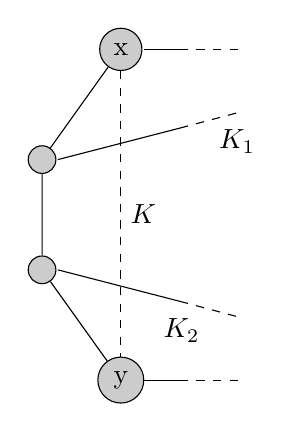
\begin{tikzpicture}[node/.style={circle,fill=black!20,draw,minimum size=1em,inner sep=3pt]}]

    \node[node] (1) at (0,0) {x};
    \node[node] (2) at (-1, -1.4)  {};
    \node[node] (3) at (-1, -2.8) {};
    \node[node] (4) at (0,-4.2) {y};

    \draw (1) -- (2) -- (3) -- (4) ;
    \draw (0.30,0) -- (0.75,0);
    \draw[dashed] (0.75, 0) -- (1.5,0);
    \draw (0.30,-4.2) -- (0.75,-4.2);
    \draw[dashed] (0.75, -4.2) -- (1.5,-4.2);
    \draw (-0.8,-1.4) -- (0.75,-1);
    \draw[dashed] (0.75, -1) to node [auto,swap] {$K_1$} (1.5,-0.8);
    \draw (-0.8,-2.8) -- (0.75,-3.2);
    \draw[dashed] (0.75, -3.2) to node [auto,swap] {$K_2$} (1.5,-3.4);
   \draw[dashed] (1) to  node [auto] {$K$} (4);

\end{tikzpicture}
\caption{Znázornění, čemu odpovídá kružnice v grafu konfliktů. Nalevo od K je část A, napravo je část B.}
\end{figure}
\end{lemma}
Struktura v klastrovém grafu, která odpovídá kružnici v grafu konfliktů se jinými slovy \uv{chová slušně a není divoce rozházená po grafu}.
\begin{proof}
Sporem předpokládejme, že v části, kde jsou klastry $K_1$ a $K_2$, je ještě jeden jiný klastr $K_3$. Uvažujme procházku z $K_1$ do $K_2$ cestou neobsahující $K$ (tedy přes $K_3$). Prvním krokem se z $K_1$ dostaneme do druhé části. Po cestě ale musíme se vrátit zpět do první části kvůli klastru $K_3$ pomocí klastru $K_i$ dříve, než se vrátíme pomocí klastru $K_2$. Klastr $K_i$ ale musí být v konfliktu s klastrem $K$, což je spor s tím, že K má jen sousedy $K_1$ a $K_2$, $K_i$ by podle všeho též musel být sousedem $K$. 
\end{proof}

\begin{tvr}
\label{lich_kruz}
Graf konfliktů obsahuje lichou kružnici $\implies$ instance (G,C) obsahuje zakázaný minor $C_6^Z$.
\end{tvr}
\begin{proof}
Důkaz indukcí podle velikosti liché kružnice. V základu indukce ukážeme, že liché kružnici velikosti 3 v grafu konfliktů odpovídá $C_6^Z$ a v indukčním kroku, pak pomocí minorových operací zredukujeme velikost podgrafu odpovídající liché kružnici o dva klastry. 

Základ indukce: Mějme trojcyklus v grafu konfliktů. Mějme příslušné klastry $\{x_1, x_2\},\{y_1, y_2\},\{z_1, z_2\}$ Podle definice konfliktů máme následující pořadí vrcholů:

Podle konfliktu klastrů $\{x_1, x_2\},\{y_1, y_2\}$ je pořádí $x_1, y_1, x_2, y_2$.

Podle konfliktu klastrů $\{y_1, y_2\},\{z_1, z_2\}$ je pořádí $y_1, z_1, y_2, z_2.$.

Podle konfliktu klastrů $\{x_1, x_2\},\{z_1, z_2\}$ je pořádí $x_1, z_1, x_2, z_2$.

Dohromady máme pořadí $x_1, y_1, z_1, x_2, y_2, z_2$, což je $C_6^Z$. Základ indukce je tedy dokázaný.

Nyní předpokládejme, že chceme dokázat tvrzení pro lichou kružnici velikosti $k$, a že tvrzení platí pro kružnici o 2 menší.

Indukční krok: Podle lemmatu 1.3 máme v $(G,\mathcal C)$ strukturu konfliktních klastrů odpovídající liché kružnici v grafu konfliktů. Předpokládejme, že jsme si $(G,\mathcal C)$ zjednodušili pomocí minorových operací tak, že nemáme nic jiného než klastry získané z liché kružnice v grafu konfliktů. Provedeme následující posloupnost minorových operací. Vezměmě předělový klastr $K$. Klastry jež jsou s ním v konfliktu, můžeme sjednodit (ubyl jeden klastr). V části, kde měly vrchol jen oni, tak sdílejí hranu, tu můžeme po provedení sjednocení zkontrahovat. Vrchol vzniklý kontrakcí odebereme. Nyní se nám kružnice přerušila. Přes rozdělení nám vede klastr $K$, pro nějž máme jedinou možnost, jak jej nahradit hranou, tak to učiníme (jinými slovy, je to korektní i v nakreslené verzi). Tuto hranu můžeme rovnou zkontrahovat a vzniklý vrchol přidáme do jednoho z klastrů (opět sjednocení klastrů a ubytí druhého klastru), které s ním mají sousední vrchol. Hranu, která jej spojovala se sousedem zkontrahujeme.  Vzniklému klastrovému grafu $(G',\mathcal C')$ odpovídá v grafu konfliktů lichá kružnice o velikosti $k-2$. Tedy $(G',\mathcal C')$ obsahuje podle indukčního předpokladu $C_6^Z$ jako klastrový minor. A jelikož $(G',\mathcal C')$ je minorem $(G,\mathcal C)$, tak $C_6^Z$ je i minorem $(G,\mathcal C)$, čímž je důkaz hotov. (TODO doplnit o ilustrující obrázky)
\end{proof}

Nyní již můžeme dokázat hlavní větu této sekce
\begin{proof} věty \ref{hlavni_veta}. 

$\implies$ \\
Pokud je $(G,\mathcal C)$ klastrově rovinný, tak podle lemmatu \ref{lemma_ekv_graf_konf_kl_rov} je graf konfliktů bipartitní, což je ekvivalentní tomu, že graf konfliktů neobsahuje lichou kružnici, což je podle tvrzení \ref{lich_kruz} dává, že $(G,\mathcal C)$ neobsahuje $C_6^Z$ jako minor.

$\Longleftarrow$ \\
Dokazujme sporem, tedy $(G,\mathcal C)$ není klastrově rovinný, ale neobsahuje $C_6^Z$ jako minor. Podle lemmatu \ref{lemma_ekv_graf_konf_kl_rov} není graf konfliktů bipartitní, tedy obsahuje lichou kružnici, což podle tvrzení \ref{lich_kruz} říká, že $(G,\mathcal C)$ má jako minor $C_6^Z$, což je spor s tím, že jsme předpokladáli, že takový minor nemá.
\end{proof}

\section{Cesty s klastry velikosti 2}
Pro cesty uvedeme o něco slabší výsledek, a to že zakázaných minorů je konečně mnoho.

\begin{theorem}
Zakázaných minorů pro cesty s klastry velikosti 2 je konečně mnoho.
\end{theorem}
\begin{proof}
Mějme klastrový graf $(G[V,E],\mathcal C)$. Vezměme saturorátor S a zkoumejme graf $(G[V,E \cup S]$. V tomto grafu mají vrcholy stupeň nejvýše 3. Tudíž zde nemůže být dělení $K_5$, ale může být dělení $K_{3,3}$. (TODO příklad klastrové cesty s dělením $K_{3,3}$) Jako minor zde můžou být obě možnosti bránící rovinnosti. Nám ale stačí, že když graf má dělení $K_{3,3}$, tak má i příslušný minor $K_{3,3}$.

Stačí se ptát, jak vypadají spojnice v dělení $K_{3,3}$ a jak je můžeme zredukovat pomocí minorových operací. Pomocí minorových operací dosáhneme nejprve, že se zbavíme všeho nepotřebného, tedy vrcholů, hran a klastrů (resp. saturovaných hran) nepodílejících se na dělění $K_{3,3}$. Dále si spojnice zjednodušíme do podoby takové, že to jsou cesty, kde se střídájí hrany a klastry. Pokud totiž máme na spojnici více hran za sebou, tak pomocí kontrakcí se zbavíme nadbytečných hran. Nyní tvrdíme, že spojnice dokážeme zredukovat pomocí minorových operací do jedné z následujících 4 typů: \\ 1) jedna hrana \\ 2) jeden klastr \\ 3) klastr a hrana \\ 4) hrana, klastr a hrana

\begin{figure}[H]
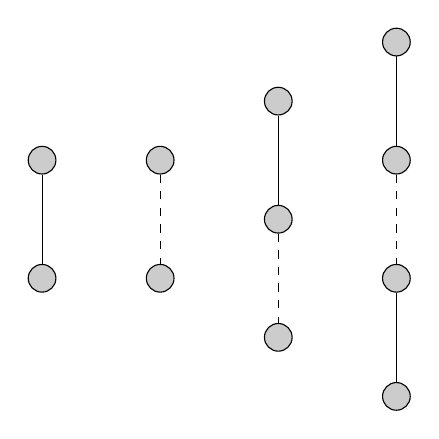
\begin{tikzpicture}[node/.style={circle,fill=black!20,draw,minimum size=1em,inner sep=3pt]}]

    \node[node] (1) at (0,0) {};
    \node[node] (2) at (0,-1.5)  {};
    \node[node] (3) at (1.5, 0) {};
    \node[node] (4) at (1.5,-1.5) {};
    \node[node] (5) at (3, 0.75) {};
    \node[node] (6) at (3, -0.75) {};
    \node[node] (7) at (3, -2.25) {};
    \node[node] (8) at (4.5, 1.5) {};
    \node[node] (9) at (4.5, 0) {};
    \node[node] (10) at (4.5,-1.5) {};
    \node[node] (11) at (4.5, -3) {};

    \draw (1) -- (2);
    \draw (5) -- (6);
    \draw (8) -- (9);
    \draw (10) -- (11);
    \draw[dashed] (3) -- (4);
    \draw[dashed] (6) -- (7);
    \draw[dashed] (9) -- (10);
\end{tikzpicture}
\caption{Typy spojnic v dělení $K_{3,3}$. Plná čára představuje hranu, čárkovaná znamená klastr.}
\end{figure}

Toho dosáhneme následovně. Pokud máme na spojnici následující situaci, že máme klastr $K_1=\{x,y\}$, hranu $e=\{y,z\}$ a klastr $K_2=\{z,w\}$ za sebou viz obrázek \ref{situace}, tak sjednotíme klastry $K_1$ a $K_2$. Ty spojuje právě jedna hrana, takže sjednocení můžeme provést bez problémů. Nyní jen vyhodíme vrcholy $y$ a $z$  a zbyde nám jen klastr $\{x,w\}$. Opakováním tohoto postupu, každou spojnici zredukujeme na jeden z čtyř výše uvedených typů.  Grafů, jenž jsou dělením $K_{3,3}$ a mají tyto typy spojnic, je konečně mnoho
\end{proof}

\begin{figure}[H]
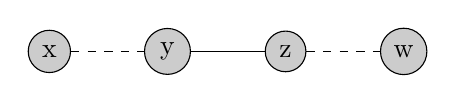
\begin{tikzpicture}[node/.style={circle,fill=black!20,draw,minimum size=1em,inner sep=3pt]}]

    \node[node] (1) at (0,0) {x};
    \node[node] (2) at (1.5,0)  {y};
    \node[node] (3) at (3, 0) {z};
    \node[node] (4) at (4.5,0) {w};

    \draw (2) -- (3);
    \draw[dashed] (1) -- (2);
    \draw[dashed] (3) -- (4);
\end{tikzpicture}
\caption{Hledaná struktura, která jde zjednodušit pomocí minorových operací}
\label{situace}
\end{figure}